\documentclass[14pt,a4paper]{article}
\usepackage[utf8]{inputenc}
\usepackage[czech]{babel}
\usepackage[T1]{fontenc}
\usepackage{amsmath}
\usepackage{amsfonts}
\usepackage{amssymb}
\usepackage{graphicx}
\usepackage{hyperref}
\usepackage{geometry}
\usepackage{float}
\usepackage{bm}
\usepackage{xcolor}
\hypersetup{
    colorlinks,
    linkcolor={red!10!black},
    citecolor={blue!50!black},
    urlcolor={blue!60!black}
}
\newtheorem{priklad}{Rovnice:}[section]
\newtheorem{poznamka}[priklad]{Poznámka}
\newtheorem{pozorovani}[priklad]{Závěr}
\title{Saxon Bowl-IYPT 2020}
\author{Kudlankográl GCHD}
\date{}
\makeatletter
\newcommand{\settitle}{\@maketitle}
\makeatother

\begin{document}
\settitle
\thispagestyle{empty}
\addtocounter{page}{-1}


\begin{figure}[H]
\centering
    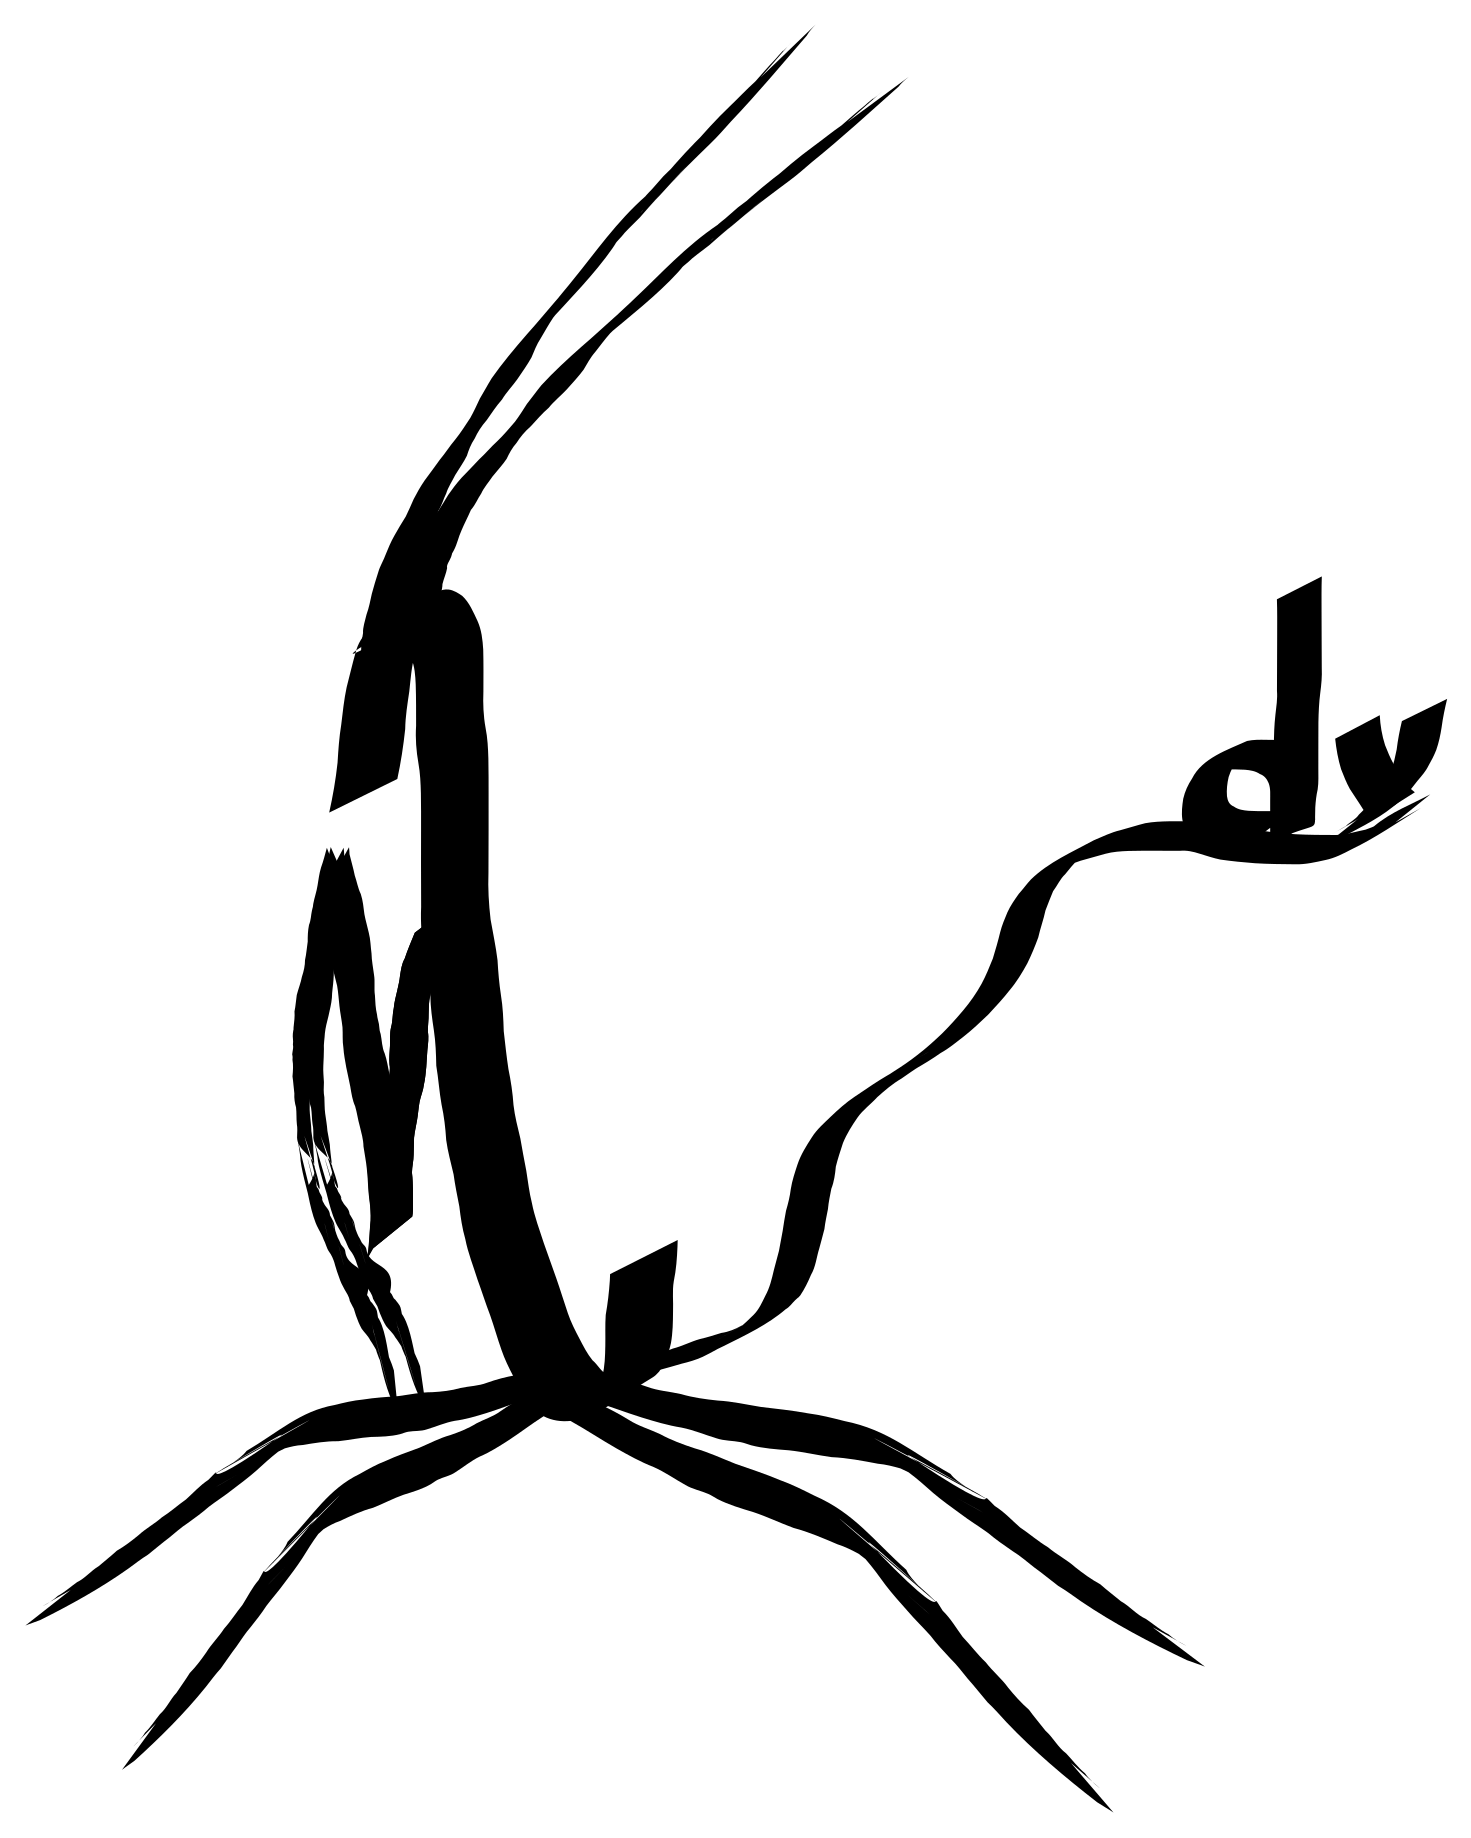
\includegraphics[width=0.76\textwidth]{kudlankogral.png}
\end{figure}

\paragraph{}
Název družstva: Kudlankográl GCHD
\paragraph{}
Škola: Gymnázium Christiana Dopplera
\paragraph{}
Adresa: Zborovská 621/45, Praha 5 - Malá Strana, 150 00

\clearpage
\newpage
\author{}
\maketitle
\thispagestyle{empty}
\tableofcontents
\newpage
\section{Úvod}
\label{sekce uvod}
\subsection{Zadání}
\paragraph{6. Saxon Bowl}
A bowl with a hole in its base will sink when placed in water. The Saxons used this device for timing purposes. Investigate the parameters that determine the time of sinking.
\paragraph{6. Saská miska}
Miska s otvorem ve dně se po vložení do vody potopí. Sasové používali toto zařízení k měření času. Prozkoumejte parametry, které určují dobu, za niž dojde k potopení.
\subsection{Vymezení obsahu řešení úlohy}
Jako náplň úlohy jsme si dali za cíl co nejpřesněji předpovědět dobu k potopení nádoby a vyvodit z toho závislosti na jednotlivých parametrech.
Zabývali jsme se závislostí na průřezu díry, hmotností nádoby, ale i na její velikosti a tvaru. Inspirovali jsme se tímto článkem: \cite{1} a jelikož nám přišla závislost na průřezu již dostatečně prozkoumaná, věnovali jsme se proto více jiným závislostem. Věříme, že k nalezení některých závislostí bude třeba počítat i teoreticky.
\newpage
\section{Experimentální část}
\subsection{Důležitá úvodní pozorování}
\paragraph{První experimenty}
Položili jsme jemně malý lehký květináč na vodní hladinu, pustili jsme ho a pozorovali, co se stane. Nejprve se moc nechtěl potápět, povrchové napětí drželo květináč na vodě skoro minutu. Pak se začal velice nesymetricky zaplavovat vodou. Na materiálu bylo vidět, že je hodně špatně smáčivý.
\begin{pozorovani}
U menších průřezů díry či u nižších hmotnosti je důležité zvolit dobře smáčivý materiál.
\end{pozorovani} 
Květináč se zprvu kymácel, až se ale naplnil o poznání více, stabilizoval se.
\begin{pozorovani}
U nižších hmotností je lepší mít jen jednu, centrální, díru nebo nádobu dostatečně zatěžkat.
\end{pozorovani} 
Hladina vody uvnitř začala růst. Zároveň i rostla hladina zvenku. Bylo rozhodně vidět, že se výšky hladin nerovnají. Hladina uvnitř se sice chce srovnat s vnější hladinou, kvůli rozdílu hydrostatických tlaků, ale zároveň květináč klesá a vnitřní hladina to nestíhá. 
\begin{pozorovani}
Vnější a vnitřní hladina vody si rozhodně nejsou rovny.
\end{pozorovani} 
Vnější hladina už dosáhla horního okraje nádoby. Vnitřní k tomu má ještě daleko. Už by se měl květináč každou chvíli potopit, ale pořád drží. Drží ho povrchové napětí, které ohnulo hladinu, tak, že je hladina sice výše než okraj květináče, ale nepřetéká dovnitř.
\begin{pozorovani}
\label{konec napeti}
Nádobu na konci opět podrží povrchové napětí. Jedná se jen o chvilku. není v našich silách ho nezahrnout do měřeného času. Bude to první zanedbaný jev, který nám pokřiví výsledky.
\end{pozorovani} 
\begin{pozorovani}
\label{konec}
Ani na konci nedojde ke srovnání hladin. Vnější hladina se prostě přelije dovnitř. V rámci předpovědi budeme uvažovat jako koncovou podmínku, jen když vnější hladina dosáhne okraje nádoby.
\end{pozorovani}
Přidali jsme závaží a zkusili jsme experiment opakovat.
Opět jsme položili nádobu na hladinu a pustili. Tentokrát už byl povrch smočený a voda se rovnoměrně rozlévala. Po puštění ale nádobka stihla zrychlit a do vody "žuchla", trochu se ještě pohoupala nahoru a dolu a až pak se stabilizovala. 
\begin{pozorovani}
\label{vyska}
Nádobu budeme spouštět právě z takové výšky, v jaké by plavala, kdyby nebylo díry. Tím zajistíme, že na začátku nebudou žádné skoky ve zrychlování.
\end{pozorovani}
\subsection{Vlastní měření}
Během pozorování se ukázalo, že nemá cenu více zvyšovat hmotnost, jelikož je pak experiment příliš krátký. Ubírání hmotností také způsobuje potíže. Nádoba pak po zaplavení i nadále plavala. To je způsobeno vlastním objemem(vztlakem) prázdné nádoby, jejíž hustota je o trochu nižší, nežli hustota vody. Zároveň musí být závaží  rovnoměrně rozložena kolem středu.\\
Následující měření byla alespoň 5-krát opakována, do tabulky je zapsána průměrná doba, než došlo k potopení nádoby.
\newpage
\subsubsection{Válec}
\label{mereni valec}
\paragraph{Měnění průřezu díry a hmotnosti nádoby}\mbox{}\\
\begin{tabular}{|c|c|c|}
\hline 
Poloměr kruhové díry$[cm]$&Hmotnost prázdné nádobky$[g]$&naměřený čas $[s]$\\ 
\hline 
\hline 
1 & 245 & 10,25\\ 
\hline 
0,8 & 245 & 15\\ 
\hline 
0,5 & 245 & 33,2\\ 
\hline 
1 & 485 & 6,1\\ 
\hline 
0,8 & 485 & 8,7\\ 
\hline 
0,5 & 485 & 19,5\\ 
\hline 
\end{tabular}
\\
\begin{tabular}{|c|c|c|}
\hline 
Strana čtvercové díry$[cm]$&Hmotnost prázdné nádobky$[g]$&naměřený čas $[s]$\\ 
\hline 
\hline 
1 & 245 & 28,92\\ 
\hline 
1,2 & 245 & 23,98\\ 
\hline 
1,5 & 245 & 15,54\\ 
\hline 
2,05 & 245 & 8,56\\ 
\hline 
1 & 485 & 15,0\\ 
\hline 
1,2 & 485 & 13,2\\ 
\hline 
1,5 & 485 & 8,7\\ 
\hline 
2,05 & 485 & 4,32\\ 
\hline 
\end{tabular}
\\\\Poloměr nádoby: $r=11,5cm$, výška nádoby: $h_{crit}=13cm$.$\uparrow$
\paragraph{Měnění "Délky" díry}\mbox{}
\\Zkoušeli jsme pod díru dát malou trubku ($5;10 cm$) a opakovali některá měření. Výsledky byly velice podobné, nejednotné odchylky mohli být způsobeny chybovostí měření, proto jsme se rozhodli tyto data zvrhnout, a prohlásili jsme "délku" díry za zanedbatelnou. Nanejvýš je to hmotnost navíc. Můžeme proto začít měření s trychtýři. 
\subsubsection{Trychtýře}
\label{mereni trychtyr}
\paragraph{Měnění průřezu díry a hmotnosti nádoby}\mbox{}\\
\begin{tabular}{|c|c|c|}
\hline 
Poloměr kruhové díry$[cm]$&Hmotnost prázdné nádoby$[g]$&naměřený čas $[s]$\\ 
\hline 
\hline 
0,45 & 66 & 11,35\\ 
\hline 
0,45 & 46 & 16,35\\ 
\hline 
0,45 & 26 & plave\\ 
\hline 
0,55 & 64,5 & 8,0\\ 
\hline 
0,55 & 44,5 & 11,0\\ 
\hline 
0,55 & 34,5 & 18,37\\ 
\hline 
0,55 & 24,5 & plave\\ 
\hline 
0,625 & 63 & 6,15\\ 
\hline 
0,625 & 43 & 9,1\\ 
\hline 
0,625 & 23 & plave\\ 
\hline 
\end{tabular}
\\Horní poloměr nádoby: $r_{max}=4,75cm$, výška nádoby: $h_{crit}=7,5cm$. $\uparrow$ \\\\
\begin{tabular}{|c|c|c|}
\hline 
Poloměr kruhové díry$[cm]$&Hmotnost prázdné nádoby$[g]$&naměřený čas $[s]$\\ 
\hline 
\hline 
0,25 & 59 & 14,15\\ 
\hline 
0,25 & 39 & 18,5\\ 
\hline 
0,25 & 19 & plave\\ 
\hline 
\end{tabular}
\\Horní poloměr nádoby: $r_{max}=3,75cm$, výška nádoby: $h_{crit}=6,5cm$. $\uparrow$
\newpage
\section{Teoretická část}
\subsection{Obecný úvod}
S využitím úvodních pozorování se teď pokusíme co nejpřesněji analyticky popsat děj.\\
\begin{figure}[H]
\centering
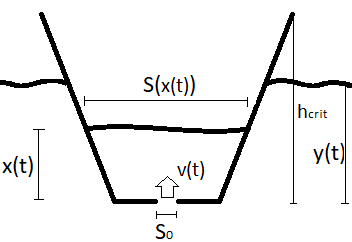
\includegraphics[scale=0.8]{Nakres.png}
\caption{Nákres, kde $v(t)$ je funkce udávající aktuální rychlost protékající vody v čase $t$. $S_0$ je průřez díry. $x(t)$ udává aktuální výšku vnitřní hladiny, $y(t)$ vnější výšku hladiny, $s(x(t))$ udává průřez nádobou ve výšce vnitřní hladiny vody a $h_{crit}$ udává celkovou výšku nádoby.}
\label{nakres}
\end{figure}
\paragraph*{•}
Děj budeme popisovat z hlediska neinerciální vztažné soustavy.
\paragraph*{•}
První rovnice, kterou budeme potřebovat, je rovnice kontinuity. Porovnáváme průtok skrz díru a přibývající objem vody v nádobě.
\begin{equation}
v(t)S_0=\frac{dx(t)}{dt}S(x(t))
\end{equation}
\paragraph*{•}
Druhou rovnicí je Toricelliho zákon, který lze odvodit z Bernoulliho rovnice.
\begin{equation}
2g(y(t)-x(t))=v^2(t)
\end{equation}
\paragraph*{•}
Nyní se podíváme na síly působící na nádobu. 
Jednak tu máme sílu gravitační. Pak sílu vztlakovou. Jsme si vědomi, že to znění vztlaku je speciálně pro statické děje, však dovolíme si tuto malou korekci, ve formě odporové síly, zanedbat.
Jelikož se na děj díváme z neinerciálního pohledu a nádobka z nerovnováhy gravitační a vztlakové síly akceleruje dolů, tak tu působí zdánlivá, setrvačná síla nádoby (ve směru nahoru). Abychom mohli v této síle uvažovat jen s hmotností prázdné nádobky, budeme muset uvažovat ztrátu hybnosti vody, která do nádobky vyvěrá.
$$F_g=F_{vz}+F_{hyb}+F_{setr}$$ 
Pro určení této síly, vycházejme ze vztahu pro nárůst hybnosti. 
$$Ft=mv \rightarrow F=mv/t=\rho Qv=\rho S v^2$$
Kde tedy prohlasme, že $v \rightarrow v(t)$ je aktuální rychlost vody protékající dírou, $S \rightarrow S_0$ je průřez této díry a $\rho$ je hustota vody (či jiné tekutiny, ve které se provádí experiment). Pak tedy:
\begin{equation}
g\left(\rho\int_{0}^{x(t)} S(z)dz+m_{misky}\right)=g \rho \int_{0}^{y(t)} S_2(z)dz+\rho S_0v^2(t)+m \frac{d^2y(t)}{dt^2}
\end{equation}
 ,kde $g$ je gravitační zrychlení a $S_2(z)$ je průřez nádobou ve výšce $z$, ale na rozdíl od $S(z)$, včetně tloušťky nádoby.
\paragraph*{•}
Počáteční hodnota pro $x(t)$ je $x(0)=0$.\\
Počáteční hodnota pro $y(t)$ je $y(0)=a$, kde $a$ bylo zadefinováno v závěru \ref{vyska} na straně \pageref{vyska}, respektive $g \rho \int_{0}^{a} S_2(z)dz=gm_{misky}$. A jak bylo řečeno v závěru \ref{konec} na straně \pageref{konec}, tak hledáme takové $t_{crit}$ pro které platí, že $y(t_{crit})=h_{crit}$.
\subsection{Zkontrolování některých vztahů}
Druhá rovnice by se dala zpochybnit, že bude platit pouze pro ideální tekutiny, proto jsme se ji rozhodli ověřit pomocí následujícího experimentu. Domníváme se, že by tento výtokový koeficient mohl být jiný (nižší) při výtoku do vodu nežli do vzduchu. Prováděli jsme experiment proto s oběma prostředími.
\subsubsection{Měření výtokového koeficientu}
Vzali jsme vysokou plastovou válcovitou nádobu, vyvrtali do ní zboku díru a nalili do nádoby vodu. Spolu s velice přesnými hodinkami a značkami na nádobce jsme natáčeli na vysokorychlostní kameru. Při měření výtokového koeficientu do vody jsme nastavili okolní hladinu na střed dírky nádoby. Ze záběrů jsme změřili čas potřebný ke změně hladiny z jedné značky na druhou. Zároveň jsme předpověděli tuto dobu pomocí následujícího vztahu:
\begin{equation}
\bm{\mathit{\Delta}} t=\frac{A}{B}\sqrt{\frac{2}{g}}\left(\sqrt{h_1}-\sqrt{h_2}\right) \quad \cite{3}
\end{equation}
\subparagraph{}
,kde $A$ je průřez válcem, $B$ je průřez dírou, $g$ je grav. zrychlení, $h_1$ původní výška a $h_2$ je nově nabytá (nižší) výška.\\
A jelikož výtokový koeficient je definovaný, jako:
\begin{equation*}
C_d=v_{skutecna}/v_{predpovezena} \quad \cite{2}
\end{equation*}
Tak pak:   \quad \quad \quad \quad 
\begin{equation}
C_d=t_{predpovezeny}/t_{skutecny}
\label{rovnice vytok}
\end{equation}
\label{mereni vytok}
\newpage
\paragraph{}
Výsledky měření:
\begin{center}
\begin{large}
Do vzduchu: ($r=0,3cm$;$r_{nadoby}=4,2cm$)\\
\end{large}
\begin{tabular}{|ccc|c|c||c||}
\hline 
$h_1 [cm]$&=>&$h_2 [cm]$& naměřený čas $[s]$& vypočítaný čas $[s]$ & $C_d$\\ 
\hline 
\hline 
7 &=>& 5 & 5,5 & 3,62 & 0,658\\ 
\hline 
7 &=>& 3 & 12,5 & 8,08 & 0,646\\ 
\hline 
7 &=>& 1 & 23,3 & 14,50 & 0,622\\ 
\hline 
5 &=>& 3 & 7,0 & 4,46 & 0,637\\ 
\hline 
5 &=>& 1 & 18,0 & 10,93& 0,607\\ 
\hline 
3 &=>& 1 & 11,0 & 6,47 & 0,588\\ 
\hline 
\hline 
&&  &  & průměr: & 0,626\\ 
\hline 
\end{tabular}
\end{center}
\begin{center}
\begin{large}
Do vody: ($r=0,3cm$;$r_{nadoby}=4,2cm$)\\
\end{large}
\begin{tabular}{|ccc|c|c||c||}
\hline 
$h_1 [cm]$&=>&$h_2 [cm]$& naměřený čas $[s]$& vypočítaný čas $[s]$ & $C_d$\\ 
\hline 
\hline 
7 &=>& 5 & 5,45 & 3,625 & 0,665\\ 
\hline 
7 &=>& 3 & 12,66 & 8,08 & 0,639\\ 
\hline 
7 &=>& 1 & 22,61 & 14,56 & 0,644\\ 
\hline 
5 &=>& 3 & 7,21 & 4,46 & 0,618\\ 
\hline 
5 &=>& 1 & 17,16 & 10,93& 0,637\\ 
\hline 
3 &=>& 1 & 9,91,0 & 6,48 & 0,651\\ 
\hline 
7 &=>& 5 & 5,73 & 3,62 & 0,633\\ 
\hline 
7 &=>& 3 & 12,71 & 8,08 & 0,636\\ 
\hline 
7 &=>& 1 & 22,53 & 14,50 & 0,646\\ 
\hline 
5 &=>& 3 & 6,98 & 4,46 & 0,638\\ 
\hline 
5 &=>& 1 & 16,80 & 10,93& 0,650\\ 
\hline 
3 &=>& 1 & 9,82 & 6,47 & 0,660\\ 
\hline 
\hline 
&&  &  & průměr: & 0,643\\ 
\hline 
\end{tabular}
\end{center}
\paragraph{}
Ačkoliv jsme vyslovili hypotézu, že by výtokový koeficient do vzduchu měl být vyšší než-li do vody, zdá se, že je tomu naopak. Zdůvodnit bychom to mohli třeba kvůli povrchovému napětí, které si "nasává" vodu z láhve. Do výpočtů použijeme koeficient do vody, jelikož, kromě situace v prvních okamžicích potápění už bude v nádobě, tedy za dírou voda. 
\paragraph{} Dále jsme vyzkoušeli, jak se bude $C_d$ chovat, budeme-li mít větší díru.:
\begin{center}
\begin{large}
Do vody, větší průřez díry($r=0,575cm$;$r_{nadoby}=4,2cm$):
\end{large}
\begin{tabular}{|ccc|c|c||c||}
\hline 
$h_1 [cm]$&=>&$h_2 [cm]$& naměřený čas $[s]$& vypočítaný čas $[s]$ & $C_d$\\ 
\hline 
\hline 
7 &=>& 5 & 1,49 & 0,99 & 0,664\\ 
\hline 
7 &=>& 3 & 3,75 & 2,20 & 0,587\\ 
\hline 
7 &=>& 1 & 7,21 & 3,96 & 0,550\\ 
\hline 
5 &=>& 3 & 2,26 & 1,21 & 0,535\\ 
\hline 
5 &=>& 1 & 5,72 & 2,98& 0,520\\ 
\hline 
3 &=>& 1 & 3,46 & 1,76 & 0,509\\ 
\hline 
7 &=>& 5 & 1,49 & 0,99 & 0,664\\ 
\hline 
7 &=>& 3 & 3,50 & 2,20 & 0,629\\ 
\hline 
7 &=>& 1 & 6,46 & 3,96 & 0,613\\ 
\hline 
5 &=>& 3 & 2,01 & 1,21 & 0,602\\ 
\hline 
5 &=>& 1 & 5,14 & 2,98& 0,580\\ 
\hline 
3 &=>& 1 & 3,13 & 1,76 & 0,562\\ 
\hline 
\hline 
&&  &  & průměr: & 0,585\\ 
\hline 
\end{tabular}
\end{center}
U tohoto měření lze očekávat větší odchylky, jelikož bylo kratší. I tak jsou ale výsledky dosti znepokojující. Je zřejmé, že se v budoucnosti budeme muset více věnovat měření $C_d$. 
\subsubsection{Závěr měření výtokového koeficientu}
\paragraph{•}
Zdroj \cite{2} udává, že by výtokový koeficient se měl nacházet někde kolem hodnoty $0,65$. Naše výsledky nemají k tomuto číslu daleko. Lze tvrdit, že se shodujeme.
\paragraph{•}
Domnívali jsme se ale, taky kvůli zdroji: \cite{2}, že by výtokový koeficient měl u větších průřezů být vyšší, výsledky měření můžeme odůvodnit nepřesností změření průměrů nádoby i díry, které nám výsledek posunuli. Proto zatím budeme všude uvažovat s $C_d=0,643$, než se tato otázka vyřeší přesněji.
\paragraph{•}
Nyní můžeme opravit druhou rovnici, aby reflektovala skutečnou rychlost proudu. Stačí dosadit za $v(t) \rightarrow v(t)/C_d$, kde $v(t)$ po dosazení už je rychlost skutečná. Tato oprava se bude týkat i třetí rovnice, ale nikoliv první, tam chceme porovnávat skutečný průtok. Zde je tedy celá, opravená soustava rovnic, kde $C_d$ je výtokový koeficient.

\begin{gather} 
v(t)S_0=\frac{dx(t)}{dt}S(x(t))\\
2g(y(t)-x(t))=\left(\frac{v(t)}{C_d}\right)^2\\
g\left(\rho\int_{0}^{x(t)} S(z)dz+m_{misky}\right)=g \rho \int_{0}^{y(t)} S_2(z)dz+\rho S_0\left(\frac{v(t)}{C_d}\right)^2+m \frac{d^2y(t)}{dt^2}
\end{gather}
$x(0)=0$, $y(0)=a$, kde pro $a$ platí 
\begin{equation}
\label{a}
g \rho \int_{0}^{a} S_2(z)dz=gm_{misky}
\end{equation}a z rovnice $y(t_{crit})=h_{crit}$ získáme $t_{crit}$, což je výstupem celého tohoto výpočtu.
\label{Final rce}
\subsection{Finální vztahy pro předpovězený čas}
\subsubsection{Pro válec}
Pro dokonalý válec platí, že $S(z)=\pi r^2$.\\
V rámci zjednodušení výpočtu, jsme se rozhodli zanedbat tloušťku plastu (tedy $S_2(z)=S(z)$). Pak:\\\\
\label{vztah valec}
$$t_{crit}=\left(h_{crit}-\frac{m_{misky}}{\rho \pi r^{2}}\right) \frac{\pi r^{2}}{C_d} \sqrt{\frac{\rho}{m_{misky g} S_0}\left(\frac{\pi r^{2}}{2S_0}+1\right)}$$
Odvození tohoto vztahu najdete v \ref{rovnice valec} na straně \pageref{rovnice valec}.\\
Když se ale podíváme na člen $\left(\frac{\pi r^2}{2S_0}+1\right)$ a zkusíme si dosadit konkrétní čísla pro poloměr a průřez díry, zjistíme, že je ta "$+1$" úplně zanedbatelná, jelikož druhý člen v závorce dosahuje čísel řádově tisíců. To bude platit dokud poloměr díry$<<$poloměr válce.
Pěkné je, že výtokový koeficient se nachází právě ve formě $\frac{1}{C_d}$, přesně jako podle rovnice \ref{rovnice vytok} v kapitole \ref{mereni vytok}.
\subsubsection{Pro trychtýře}
\label{vztah trychtyr}
Pro kruhový trychtýř platí, že $S(z)=\pi tg^2(\alpha)z^2$, kde $\alpha$ je vnitřní úhel mezi osou a stěnou trychtýře.Opět jsme se rozhodli zanedbat tloušťku plastu (tedy $S_2(z)=S(z)$). $\alpha$ jsme spočítali jako $\alpha=arctg(r_{max}/h_{crit})$\\\\
U trychtýřů jsme se rozhodli dělat numerickou simulaci, jednak pro zpestření, ale taky proto, že by naše diferenciální rovnice s minimem aproximací byly neřešitelné. (nebyly by ani "ordinary", ani separovatelné).
Hlavními vzorci na výpočet jednotlivých iteračních kroků jsou : $$v_i=C_d\sqrt{2g(y_{i-1}-x_{i-1})}$$$$ \downarrow$$ 
$$x_i=\sqrt[3]{\frac{3S_0}{\pi tg^2(\alpha)} \left(v_idt+\frac{\pi tg^2(\alpha)}{3S_0}x_{i-1}^{3}\right)}$$$$ \downarrow$$ 
$$dy_i=\frac{\frac{m_{misky}}{\rho}-\frac{\pi tg^{2}(\alpha)}{3}\left(x^{3}_{i-1}-y^{3}_{i-1}\right)-\rho S_0\left(\frac{v(t)}{C_d}\right)^2}{m_{misky}}dt+dy_{i-1}$$ 
$$ \downarrow$$ 
$$y_i=dy_i*dt+y_{i-1}$$
\begin{center}
a tedy samozřejmě:
\end{center} 
$$t_i=t_{i-1}+dt$$
,kde $dt$ je velikost iteračního kroku a $dy$ je přírustek na $y$ za $dt$ (tedy derivace jeho).\\
Princip simulace a odvození těchto vzorců najdete rozepsaný v \ref{rovnice trychtyr} na straně \pageref{rovnice trychtyr}.







\subsection{Porovnání výsledků}
Pro válcovitou nádobu zkopírováním dat z \ref{mereni valec} na straně \pageref{mereni valec} a s přidáním dat s využitím finálního vzorce z \ref{vztah valec} na straně \pageref{vztah valec} dostáváme tuto finální tabulku, $C_d=0,643$:\\
\begin{tabular}{|c|c||c|c||}
\hline 
Poloměr kruhové díry$[cm]$&Hmotnost prázdné nádobky$[g]$&naměřený čas $[s]$&vypočítaný čas $[s]$\\ 
\hline 
\hline 
1 & 245 & 10,25 & 8,280\\ 
\hline 
0,8 & 245 & 15& 12,804\\ 
\hline 
0,5 & 245 & 33,2& 32,407\\ 
\hline 
1 & 485 & 6,1& 4,606\\ 
\hline 
0,8 & 485 & 8,7& 7,123\\ 
\hline 
0,5 & 485 & 19,5& 18,027\\ 
\hline 
\end{tabular}
\\
\begin{tabular}{|c|c||c|c||}
\hline 
Strana čtvercové díry$[cm]$&Hmotnost prázdné nádobky$[g]$&naměřený čas $[s]$&vypočítaný čas $[s]$\\ 
\hline 
\hline 
1 & 245 & 28,92& 25,489\\ 
\hline 
1,2 & 245 & 23,98& 17,774\\ 
\hline 
1,5 & 245 & 15,54& 11,461\\ 
\hline 
2,05 & 245 & 8,56& 4,276\\ 
\hline 
1 & 485 & 15,0& 14,197\\ 
\hline 
1,2 & 485 & 13,2& 9,888\\ 
\hline 
1,5 & 485 & 8,7& 6,376\\ 
\hline 
2,05 & 485 & 4,32& 2,379\\ 
\hline 
\end{tabular}
Zaneseme-li změřená data a vypočítaná data (však pro více hodnot, aby nám mohla vzniknout hezčí křivka) tak dostáváme následující graf.:
\begin{figure}[H]
\centering
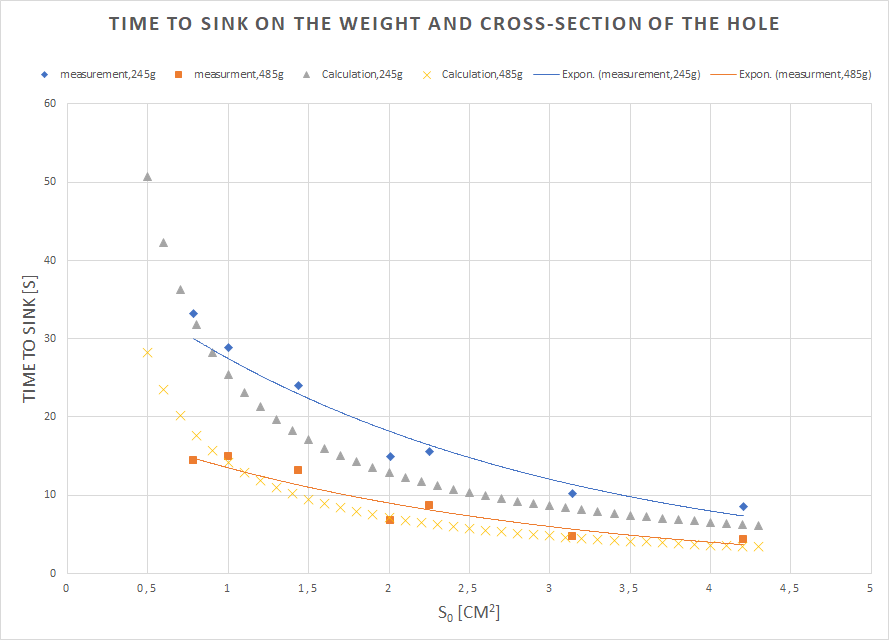
\includegraphics[scale=0.6]{Tabulka2.png}
\label{nakres}
\end{figure}
Pro naše trychtýře, kopírováním dat z \ref{mereni trychtyr} na straně \pageref{mereni trychtyr} a přidání výsledků ze simulací (viz \ref{vztah trychtyr}, dostáváme tuto tabulku:\\
\begin{tabular}{|c|c||c|c||}
\hline 
Poloměr kruhové díry$[cm]$&Hmotnost prázdné nádoby$[g]$&naměřený čas $[s]$&nasimulovaný čas $[s]$\\ 
\hline 
\hline 
0,45 & 66 & 11,35 & 10,9\\ 
\hline 
0,45 & 46 & 16,35 & 16,14\\ 
\hline 
0,45 & 26 & plave & ---\\ 
\hline 
0,55 & 64,5 & 8,0 & 7,68\\ 
\hline 
0,55 & 44,5 & 11,0 & 10,57\\ 
\hline 
0,55 & 34,5 & 18,37 & 13,22\\ 
\hline 
0,55 & 24,5 & plave & ---\\ 
\hline 
0,625 & 63 & 6,15 & 5,88\\ 
\hline 
0,625 & 43 & 9,1& 8,79\\ 
\hline 
0,625 & 23 & plave& ---\\ 
\hline 
\end{tabular}
\\Horní poloměr nádoby: $r_{max}=4,75cm$, výška nádoby: $h_{crit}=7,5cm$. $\uparrow$ \\\\
\begin{tabular}{|c|c||c|c||}
\hline 
Poloměr kruhové díry$[cm]$&Hmotnost prázdné nádoby$[g]$&naměřený čas $[s]$&nasimulovaný čas $[s]$\\ 
\hline 
\hline 
0,25 & 59 & 14,15 & 14,09\\ 
\hline 
0,25 & 39 & 18,5 & 18,34\\ 
\hline 
0,25 & 19 & plave & ---\\ 
\hline 
\end{tabular}
\\Horní poloměr nádoby: $r_{max}=3,75cm$, výška nádoby: $h_{crit}=6,5cm$. $\uparrow$
\paragraph{•}Pokud nebyla přidaná hmotnost dostatečná a nádoba se nepotápěla, plavala díky vlastnímu vztlaku, tak jelikož tento parametr nemáme započítaný, tak jsme neprováděli pro tyto parametry simulaci. Stejně lze odůvodnit velkou odchylku na šestém řádku.
\newpage
\section{Závěr a diskuze}
\subsection{Objasnění nepřesností a odchylek}
\paragraph{•}Jak bylo řečeno v závěru \ref{konec napeti} na straně \pageref{konec napeti}, několik sekund (1-3) je nádoba podle našich výpočtů potopena, i když ještě drží díky povrchovému napětí. Tento čas je menší pro větší hmotnosti.
\paragraph{•}Zanedbali jsme vlastní objem nádoby, způsobující další vztlak, viditelné hlavně u trychtýřů.
\paragraph{•}Uvažovali jsme se stacionárním archimédovským vztlakem.
\paragraph{•}Naše nádoba, kterou jsme prohlásili za válec je lehce konická, do výpočtu jako poloměr válce jsme vzali hodnotu ze středu.
\paragraph{•}Zanedbaná je i viskozita vody, která by měla čas potápění zvýšit o trochu.
\paragraph{•}Hodnota výtokového koeficientu se může různit pro jinak vytvarované díry, zatím jsme tuto malou odchylku zanedbali. 
\subsection{Rekapitulace dosažených výsledků}
\paragraph{•}Udělali jsme mnoho různých měření.
\paragraph{•}Ověřili jsme naše teorie, sice ne moc kvalitativně, ale rozhodně kvantitativně.
\paragraph{•}V rámci našich dovedností jsme dosáhli relativně dobrých předpovědí.
\paragraph{•}Vytvořili jsme model, který popisuje jev velice obecně (viz \ref{Final rce}).
\subsection{Náměty na budoucí výzkum}
\paragraph{•}Udělat více měření s měněním hmotnosti, průřezu či velikosti a tvaru nádoby.
\paragraph{•}Započítat do předpovědi některé nezapočítané prvky, jako třeba poslední sekundy před potopením, nebo vlastní vztlak prázdné nádobky.
\paragraph{•}Zkontrolovat měření výtokového koeficientu.
\paragraph{•}Více se věnovat povrchovému napětí, jako perličku.
\paragraph{•}Vytvořit grafické simulace.
\newpage
\section{Odvození vztahu z 3. oddělení.}
Sem rozepíšeme všechny odvození vzorců, která mohou být dlouhá či nezáživná.
\subsection{Pro válec}
\label{rovnice valec}
Zde je odvozeni ke vztahu, který najdete v \ref{vztah valec} na straně \pageref{vztah valec}.\\
Vycházejme z finální soustavy rovnic v \ref{Final rce} a dosaďme $S_2(z)=S(z)=\pi r^2$. \quad $\rightarrow$
\begin{gather} 
\label{9}
v(t)S_0=\frac{dx(t)}{dt}\pi r^2\\
\label{10}
2g(y(t)-x(t))=\left(\frac{v(t)}{C_d}\right)^2\\
\label{11}
g\left(\rho\pi r^2x(t)+m_{misky}\right)=g \rho \pi r^2y(t)+\rho S_0\left(\frac{v(t)}{C_d}\right)^2+m \frac{d^2y(t)}{dt^2}
\end{gather}
Vyjádříme $v(t)$ z rovnice \ref{10} a dosadíme jej do rovnice \ref{9} a \ref{11}.
\begin{gather}
\label{12}
C_d\sqrt{2g(y(t)-x(t))}=\frac{dx}{dt}\frac{\pi r^2}{S_0}\\
\label{13}
g\left(\rho\pi r^2x(t)+m_{misky}\right)=g \rho \pi r^2y(t)+\rho 2S_0g(y(t)-x(t))+m \frac{d^2y(t)}{dt^2}
\end{gather}
Z \ref{13} vyjádříme $x(t)$ a dosadíme do \ref{12} a trochu upravíme:
\begin{equation}
C_d\sqrt{\frac{2gm_{misky}}{\rho \left(\pi r^{2}+2S_0\right)}\left(1-\frac{d^{2}y(t)}{gdt^{2}}\right)}=\frac{\pi r^2}{S_0}\left(\frac{dy(t)}{dt}+\frac{m_{misky}}{g\rho (\pi r^{2}+2S_0)}\frac{d^3y(t)}{dt^3}\right)
\end{equation}
Tato rovnice nevypadá řešitelně, leda bychom udělali drobnou aproximaci. Z pozorování potápění nádoby jsme si dosti jistí a také díky tomu, že nádoba začíná v právě takové výšce, v jaké by plavala (\ref{vyska}), tak jsme si jistí, že $d^{2}y(t)/dt^{2}$ je velice blízko nule. Proto můžeme si dovolit, $\sqrt{1-\frac{d^{2}y(t)}{gdt^{2}}} \rightarrow \left(1-\frac{d^{2}y(t)}{2gdt^{2}}\right)$. Dostáváme se tím na obyčejnou nehomogenní diferenciální rovnici 3. stupně. Jednoduchou substitucí snížíme rovnici o jeden řád.
\begin{gather}
\label{15}
\left| \frac{dy(t)}{dt}=v(t)\right| \rightarrow\\
\label{16}
C_d\sqrt{\frac{2gm_{misky}}{\rho \left(\pi r^{2}+2S_0\right)}}=\frac{\pi r^2}{S_0}v(t)+\frac{dv(t)}{2gdt}+\frac{m_{misky}\pi r^2}{\rho S_0(\pi r^{2}+2S_0)}\frac{d^{2}y(t)}{dt^{2}}
\end{gather}
Jak jistě víme,obecným řešením obyčejné nehomogenní dif. rovnice je obecné řešení této rovnice, ale homogenní $+$ částečné řešení této rovnice nehomogenně.
Obecným řešením homogenní rovnice je $$v(t)=c_1e^{tp_1}+c_2e^{tp_2}$$, kde $p_{1;2}$ lze dopočítat z charakteristického polynomu:$
\frac{\pi r^2}{S_0}+\frac{1}{2g}p+\frac{m_{misky}\pi r^2}{\rho S_0(\pi r^{2}+2S_0)}p^{2}=0$
To ale rovnou zanedbáme, jelikož nevyhovuje situaci. $p$ vychází komplexně, což vede na součet $sin$u a $cos$inu. Proto budeme uvažovat pouze s částečným řešením nehomogenní rovnice. Předpokládejme, že by $v(t)$ mohl být polynom až druhého stupně na $t$. Po dosazení tohoto předpokladu do rovnice \ref{16} dostáváme jako jediné možné řešení: \begin{equation*}
v(t)=\frac{S_0C_d}{\pi r^2}\sqrt{\frac{2gm_{misky}}{\rho \left(\pi r^{2}+2S_0\right)}}
\end{equation*}
Vrátíme-li se k substituci \ref{15}, tak zintegrováním tohoto získáváme:
 \begin{equation*}
y(t)=\frac{S_0C_d}{\pi r^2}\sqrt{\frac{2gm_{misky}}{\rho \left(\pi r^{2}+2S_0\right)}} t+a
\end{equation*}
,kde $a$ je počáteční hodnota pro $y(t)$ (viz rovnice \ref{a} v kapitole \ref{Final rce}). \\
Nyní vycházejme z koncové podmínky $y(t_{crit})=h_{crit}$, po troše úprav docházíme ke vztahu:
$$t_{crit}=\left(h_{crit}-\frac{m_{misky}}{\rho \pi r^{2}}\right) \frac{\pi r^2}{C_d} \sqrt{\frac{\rho}{m_{misky}gS_0}\left(\frac{\pi r^2}{2S_0}+1\right)}$$ 
\subsection{Pro trychtýř}
\label{rovnice trychtyr}
Zde je popis principu simulace, kterou najdete v \ref{vztah trychtyr} na straně \pageref{vztah trychtyr}.\\ Vycházejme z finální soustavy rovnic v \ref{Final rce} a dosaďme $S_2(z)=S(z)=\pi tg^2(\alpha)x^2(t)$. \quad $\rightarrow$
\begin{gather} 
\label{18}
v(t)S_0=\frac{dx(t)}{dt}\pi tg^2(\alpha)x^2\\
\label{19}
2g(y(t)-x(t))=\left(\frac{v(t)}{C_d}\right)^2\\
\label{20}
g\left(\rho\pi tg^2(\alpha)  \frac{x^{3}(t)}{3} +m_{misky}\right)=g \rho \pi tg^2(\alpha) \frac{y^{3}(t)}{3} +\rho S_0\left(\frac{v(t)}{C_d}\right)^2+m \frac{d^2y(t)}{dt^2}
\end{gather}
Principem numerické simulace, je uvažovat s funkcemi jako s číselnými řadami. Iterační krok nazveme $dt$. Platí, že 
\begin{equation}
t_i=t_{i-1}+dt
\end{equation}
Z rovnice \ref{19} snadno získáme vztah:
\begin{equation}
v_i=\sqrt{2g(y_{i-1}-x_{i-1})}C_d
\end{equation}
Dále můžeme snadno vyjádřit $d^{2}y_i$ z rovnice \ref{20} jako:
$$d^{2}y_i=\frac{\frac{m_{misky}}{\rho}-\frac{\pi tg^{2}(\alpha)}{3}\left(x^{3}_{i-1}-y^{3}_{i-1}\right)-\rho S_0\left(\frac{v(t)}{C_d}\right)^2}{m_{misky}}$$
, kde $d^{2}y_i$ je přírustek na přírustku na $y_i$ (prakticky druhá derivace $y$, ale v iteračním pojetí).
Vycházejíc z definice derivace, tak z $d^{2}y_i$ můžeme vyjádřit $dy_i$ jako: $$ dy_i=d^{2}y_idt+dy_{i-1}=\frac{\frac{m_{misky}}{\rho}-\frac{\pi tg^{2}(\alpha)}{3}\left(x^{3}_{i-1}-y^{3}_{i-1}\right)-\rho S_0\left(\frac{v(t)}{C_d}\right)^2}{m_{misky}}dt+dy_{i-1}$$
A tedy nápodobně:
\begin{equation}
y_i=\frac{\frac{m_{misky}}{\rho}-\frac{\pi tg^{2}(\alpha)}{3}\left(x^{3}_{i-1}-y^{3}_{i-1}\right)-\rho S_0\left(\frac{v(t)}{C_d}\right)^2}{m_{misky}}(dt)^{2}+dy_{i-1}dt+y_{i-1}
\end{equation}
S vyjádřením $x_i$ to je ale trochu složitější. Musíme se vrátit k rovnici \ref{18} a počítat zase trochu analyticky. Vyjádříme totiž z této separovatelné diferenciální rovnice $x(t)$ jako: $$x(t)=\sqrt[3]{\frac{3S_0}{\pi tg^2(\alpha)} \int_0^t v(t)dt}$$
Tento integrál budeme počítat iteračně přímo z definice Riemannova integrálu. $$\int_0^t v(t)dt \rightarrow \int_{t_{i-1}}^{t_{i}} v(t)dt + \int_{0}^{t_{i-1}} v(t)dt \simeq v_idt+\int_{0}^{t_{i-1}} v(t)dt$$ 
, kde $\int_{0}^{t_{i-1}} v(t)dt$ je plocha pod $v$ do předchozí bodu. Tu vyjádříme ve vztahu k předchozí hodnotě $x$. Dostáváme tak:
\begin{equation}
x_i=\sqrt[3]{\frac{3S_0}{\pi tg^2(\alpha)} \left(v_idt+\frac{\pi tg^2(\alpha)}{3S_0}x_{i-1}^{3}\right)}
\end{equation}
Teď už máme dost vzorců pro jednotlivé proměnné.
Ještě potřebujeme počáteční hodnoty pro $y ; x; dy;t$:\\
$x_0=0$ (viz \ref{Final rce})\\
$y_0=\sqrt[3]{\frac{3m_{misky}}{\rho \pi}}$	(viz rovnice \ref{a} v \ref{Final rce})\\
$dy_0=0$\\
$t_0=0$\\
K simulaci lze vytvořit jednoduchý program, my jsme ale pro přehlednost použili tabulkovou aplikaci-excel. Jako $dt$ jsme volili $0,01s$. Jelikož ale výsledky dosti oscilovali, vytvořili jsme další sloupec s "plovoucím průměrem". Ten vzal posledních 25 hodnot $y$ a zprůměroval je. Výsledkem byla čísla, ze kterých jsme mohli vyčíst hodnotu $t_i$ když platí, nebo byla překročena koncová podmínka $y_i=h_{crit}$.
\newpage
\section{Použitá literatura}
\begin{thebibliography}{3}
\bibitem{1}
Greer, Allan \& Kincanon, Eric. (2000). An experiment with Saxon bowls. The Physics Teacher. 38. 112-112. 10.1119/1.880442.  Dostupné z:
\href{https://www.researchgate.net/publication/239045627_An_experiment_with_Saxon_bowls}{ researchgate.net}
\bibitem{2}
Discharge Coefficient for Nozzles and Orifices – Neutrium. Neutrium [online]. Copyright © 2019 [cit. 19.12.2019]. Dostupné z:
\href{https://neutrium.net/fluid_flow/discharge-coefficient-for-nozzles-and-orifices/}{Neutrinum.net}

\bibitem{3}
T. E. Faber (1995). Fluid Dynamics for Physicists. Cambridge University Press. ISBN 978-0-521-42969-6.\\
Stanley Middleman, An Introduction to Fluid Dynamics: Principles of Analysis and Design (John Wiley \& Sons, 1997) ISBN 978-0-471-18209-2\\
Dennis G. Zill (14 May 2008). A First Course in Differential Equations. Cengage Learning. ISBN 0-495-10824-3.
\end{thebibliography}
\end{document}
